\documentclass{standalone}
\usepackage{tikz}
\usetikzlibrary{patterns, positioning}

\begin{document}
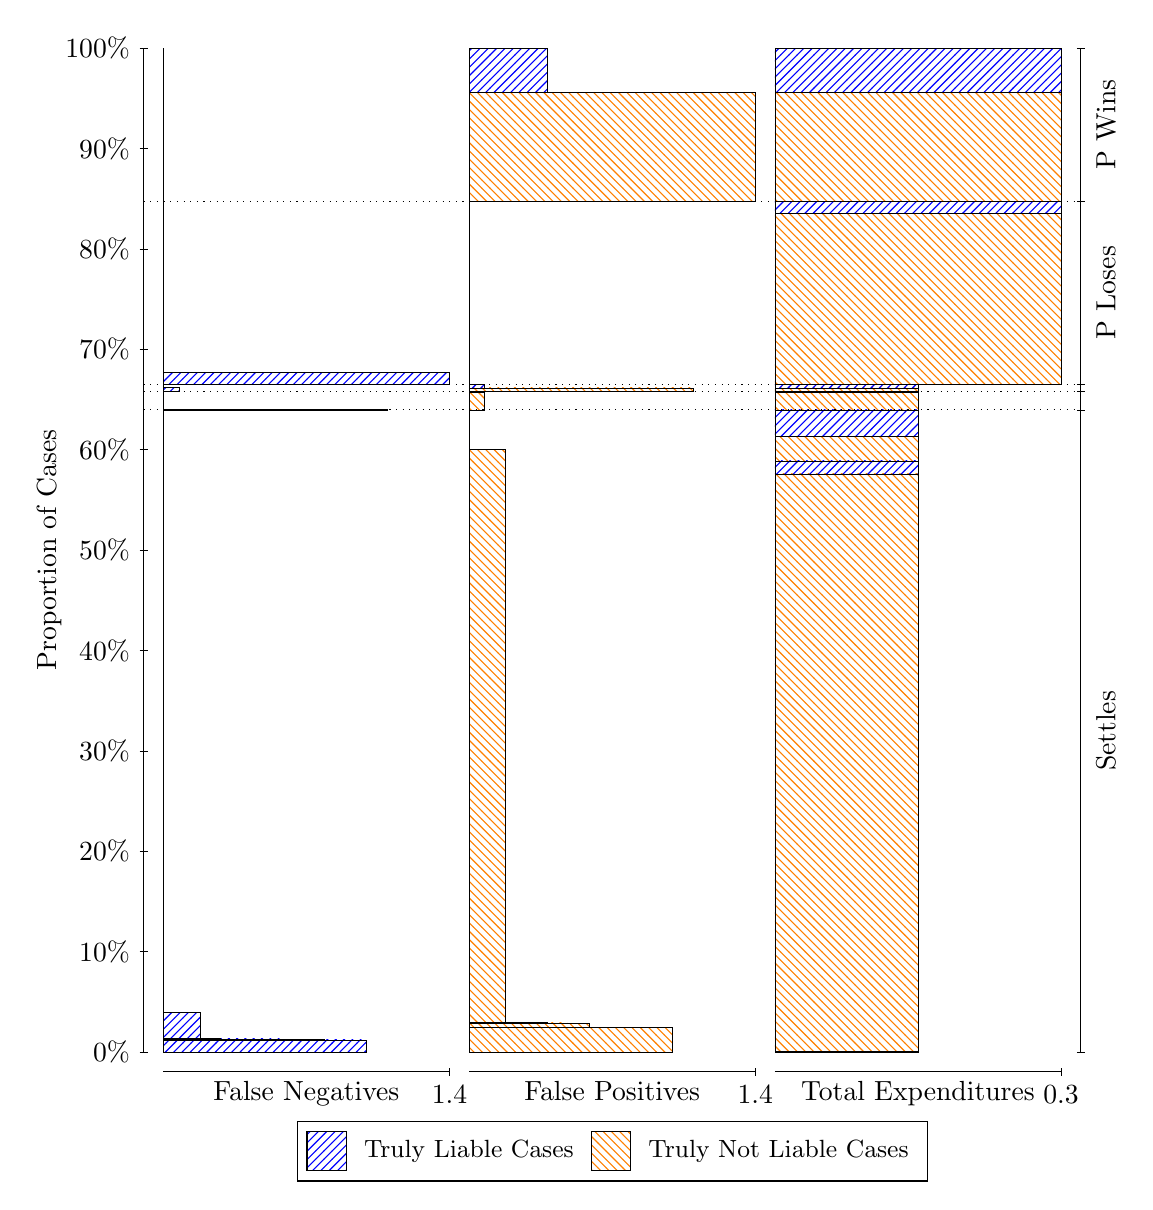
\begin{tikzpicture}
\draw[black, very thin] (1.5,1.75) -- (1.5,14.5);
\node[rotate=90, anchor=center] at (0.3, 8.125) {Proportion of Cases};
\draw[black, very thin] (1.45,1.75) -- (1.55,1.75);
\node[anchor=east] at (1.45, 1.75) {0\%};
\draw[black, very thin] (1.45,3.025) -- (1.55,3.025);
\node[anchor=east] at (1.45, 3.025) {10\%};
\draw[black, very thin] (1.45,4.3) -- (1.55,4.3);
\node[anchor=east] at (1.45, 4.3) {20\%};
\draw[black, very thin] (1.45,5.575) -- (1.55,5.575);
\node[anchor=east] at (1.45, 5.575) {30\%};
\draw[black, very thin] (1.45,6.85) -- (1.55,6.85);
\node[anchor=east] at (1.45, 6.85) {40\%};
\draw[black, very thin] (1.45,8.125) -- (1.55,8.125);
\node[anchor=east] at (1.45, 8.125) {50\%};
\draw[black, very thin] (1.45,9.4) -- (1.55,9.4);
\node[anchor=east] at (1.45, 9.4) {60\%};
\draw[black, very thin] (1.45,10.675) -- (1.55,10.675);
\node[anchor=east] at (1.45, 10.675) {70\%};
\draw[black, very thin] (1.45,11.95) -- (1.55,11.95);
\node[anchor=east] at (1.45, 11.95) {80\%};
\draw[black, very thin] (1.45,13.225) -- (1.55,13.225);
\node[anchor=east] at (1.45, 13.225) {90\%};
\draw[black, very thin] (1.45,14.5) -- (1.55,14.5);
\node[anchor=east] at (1.45, 14.5) {100\%};

\draw[black, very thin] (13.4,1.75) -- (13.4,14.5);
\draw[black, very thin] (13.35,1.75) -- (13.45,1.75);
\node[anchor=west] at (13.35, 1.75) {};
\draw[black, very thin] (13.35,9.9046) -- (13.45,9.9046);
\node[anchor=west] at (13.35, 9.9046) {};
\draw[black, very thin] (13.35,10.14) -- (13.45,10.14);
\node[anchor=west] at (13.35, 10.14) {};
\draw[black, very thin] (13.35,10.23) -- (13.45,10.23);
\node[anchor=west] at (13.35, 10.23) {};
\draw[black, very thin] (13.35,12.556) -- (13.45,12.556);
\node[anchor=west] at (13.35, 12.556) {};
\draw[black, very thin] (13.35,14.5) -- (13.45,14.5);
\node[anchor=west] at (13.35, 14.5) {};

\draw[black, very thin, pattern color=blue, pattern=north east lines] (1.75,1.75) rectangle (4.3264,1.904);
\draw[black, very thin, pattern color=blue, pattern=north east lines] (1.75,1.904) rectangle (4.0621,1.9046);
\draw[black, very thin, pattern color=blue, pattern=north east lines] (1.75,1.9046) rectangle (3.7979,1.9053);
\draw[black, very thin, pattern color=blue, pattern=north east lines] (1.75,1.9053) rectangle (3.5336,1.906);
\draw[black, very thin, pattern color=blue, pattern=north east lines] (1.75,1.906) rectangle (3.2694,1.9172);
\draw[black, very thin, pattern color=blue, pattern=north east lines] (1.75,1.9172) rectangle (3.0052,1.9174);
\draw[black, very thin, pattern color=blue, pattern=north east lines] (1.75,1.9174) rectangle (2.7409,1.9175);
\draw[black, very thin, pattern color=blue, pattern=north east lines] (1.75,1.9175) rectangle (2.4767,1.9177);
\draw[black, very thin, pattern color=blue, pattern=north east lines] (1.75,1.9177) rectangle (2.2124,2.252);
\draw[black, very thin, pattern color=orange, pattern=north west lines] (1.75,2.252) rectangle (1.75,9.9046);
\draw[black, very thin, pattern color=blue, pattern=north east lines] (1.75,9.9046) rectangle (4.5906,9.9116);
\draw[black, very thin, pattern color=orange, pattern=north west lines] (1.75,9.9116) rectangle (1.75,10.14);
\draw[black, very thin, pattern color=blue, pattern=north east lines] (1.75,10.14) rectangle (1.9482,10.187);
\draw[black, very thin, pattern color=orange, pattern=north west lines] (1.75,10.187) rectangle (1.75,10.23);
\draw[black, very thin, pattern color=blue, pattern=north east lines] (1.75,10.23) rectangle (5.3833,10.382);
\draw[black, very thin, pattern color=orange, pattern=north west lines] (1.75,10.382) rectangle (1.75,12.556);
\draw[black, very thin, pattern color=orange, pattern=north west lines] (1.75,12.556) rectangle (1.75,13.932);
\draw[black, very thin, pattern color=blue, pattern=north east lines] (1.75,13.932) rectangle (1.75,14.5);
\draw[black, very thin, pattern color=orange, pattern=north west lines] (5.6333,1.75) rectangle (8.2097,2.0616);
\draw[black, very thin, pattern color=orange, pattern=north west lines] (5.6333,2.0616) rectangle (7.9455,2.0623);
\draw[black, very thin, pattern color=orange, pattern=north west lines] (5.6333,2.0623) rectangle (7.6812,2.063);
\draw[black, very thin, pattern color=orange, pattern=north west lines] (5.6333,2.063) rectangle (7.417,2.0636);
\draw[black, very thin, pattern color=orange, pattern=north west lines] (5.6333,2.0636) rectangle (7.1527,2.1163);
\draw[black, very thin, pattern color=orange, pattern=north west lines] (5.6333,2.1163) rectangle (6.8885,2.1164);
\draw[black, very thin, pattern color=orange, pattern=north west lines] (5.6333,2.1164) rectangle (6.8885,2.1195);
\draw[black, very thin, pattern color=orange, pattern=north west lines] (5.6333,2.1195) rectangle (6.6242,2.1226);
\draw[black, very thin, pattern color=orange, pattern=north west lines] (5.6333,2.1226) rectangle (6.36,2.1255);
\draw[black, very thin, pattern color=orange, pattern=north west lines] (5.6333,2.1255) rectangle (6.0958,9.4026);
\draw[black, very thin, pattern color=blue, pattern=north east lines] (5.6333,9.4026) rectangle (5.6333,9.9046);
\draw[black, very thin, pattern color=orange, pattern=north west lines] (5.6333,9.9046) rectangle (5.8315,10.133);
\draw[black, very thin, pattern color=blue, pattern=north east lines] (5.6333,10.133) rectangle (5.6333,10.14);
\draw[black, very thin, pattern color=orange, pattern=north west lines] (5.6333,10.14) rectangle (8.4739,10.184);
\draw[black, very thin, pattern color=blue, pattern=north east lines] (5.6333,10.184) rectangle (5.8315,10.23);
\draw[black, very thin, pattern color=orange, pattern=north west lines] (5.6333,10.23) rectangle (5.6333,12.404);
\draw[black, very thin, pattern color=blue, pattern=north east lines] (5.6333,12.404) rectangle (5.6333,12.556);
\draw[black, very thin, pattern color=orange, pattern=north west lines] (5.6333,12.556) rectangle (9.2667,13.932);
\draw[black, very thin, pattern color=blue, pattern=north east lines] (5.6333,13.932) rectangle (6.6242,14.5);
\draw[black, very thin, pattern color=orange, pattern=north west lines] (9.5167,1.75) rectangle (11.333,1.7592);
\draw[black, very thin, pattern color=blue, pattern=north east lines] (9.5167,1.7592) rectangle (11.333,1.7611);
\draw[black, very thin, pattern color=orange, pattern=north west lines] (9.5167,1.7611) rectangle (11.333,9.0909);
\draw[black, very thin, pattern color=blue, pattern=north east lines] (9.5167,9.0909) rectangle (11.333,9.2561);
\draw[black, very thin, pattern color=orange, pattern=north west lines] (9.5167,9.2561) rectangle (11.333,9.5698);
\draw[black, very thin, pattern color=blue, pattern=north east lines] (9.5167,9.5698) rectangle (11.333,9.9046);
\draw[black, very thin, pattern color=orange, pattern=north west lines] (9.5167,9.9046) rectangle (11.333,10.133);
\draw[black, very thin, pattern color=blue, pattern=north east lines] (9.5167,10.133) rectangle (11.333,10.14);
\draw[black, very thin, pattern color=orange, pattern=north west lines] (9.5167,10.14) rectangle (11.333,10.184);
\draw[black, very thin, pattern color=blue, pattern=north east lines] (9.5167,10.184) rectangle (11.333,10.23);
\draw[black, very thin, pattern color=orange, pattern=north west lines] (9.5167,10.23) rectangle (13.15,12.404);
\draw[black, very thin, pattern color=blue, pattern=north east lines] (9.5167,12.404) rectangle (13.15,12.556);
\draw[black, very thin, pattern color=orange, pattern=north west lines] (9.5167,12.556) rectangle (13.15,13.932);
\draw[black, very thin, pattern color=blue, pattern=north east lines] (9.5167,13.932) rectangle (13.15,14.5);
\draw[black, dotted] (1.5,9.9046) -- (13.4,9.9046);
\draw[black, dotted] (1.5,10.14) -- (13.4,10.14);
\draw[black, dotted] (1.5,10.23) -- (13.4,10.23);
\draw[black, dotted] (1.5,12.556) -- (13.4,12.556);
\draw[black, very thin] (1.75,1.5) -- (5.3833,1.5);
\node[anchor=north] at (3.5667, 1.5) {False Negatives};
\draw[black, very thin] (5.3833,1.45) -- (5.3833,1.55);
\node[anchor=north] at (5.3833, 1.45) {1.4};

\draw[black, very thin] (5.6333,1.5) -- (9.2667,1.5);
\node[anchor=north] at (7.45, 1.5) {False Positives};
\draw[black, very thin] (9.2667,1.45) -- (9.2667,1.55);
\node[anchor=north] at (9.2667, 1.45) {1.4};

\draw[black, very thin] (9.5167,1.5) -- (13.15,1.5);
\node[anchor=north] at (11.333, 1.5) {Total Expenditures};
\draw[black, very thin] (13.15,1.45) -- (13.15,1.55);
\node[anchor=north] at (13.15, 1.45) {0.3};

\node[black, centered, rotate=90] at (13.72, 5.8273) {Settles};


\node[black, centered, rotate=90] at (13.72, 11.393) {P Loses};
\node[black, centered, rotate=90] at (13.72, 13.528) {P Wins};

\draw (7.449999999999999,1.5) node[draw=none] (baseCoordinate) {};
\begin{scope}[align=center]
        \matrix[scale=0.5, draw=black, below=0.5cm of baseCoordinate, nodes={draw}, column sep=0.1cm]{
            \node[rectangle, draw, minimum width=0.5cm, minimum height=0.5cm, pattern=north east lines, pattern color=blue] {}; &
            \node[draw=none, font=\small] (B) {Truly Liable Cases}; &
            \node[rectangle, draw, minimum width=0.5cm, minimum height=0.5cm, pattern=north west lines, pattern color=orange] {}; &
            \node[draw=none, font=\small] (B) {Truly Not Liable Cases}; \\
            };
\end{scope}

\end{tikzpicture}
\end{document}